\documentclass[10pt,letterpaper]{article}
\usepackage[margin=.77in,headheight=16pt]{geometry}
\usepackage{amsmath,amssymb,mathtools,microtype,tikz,xcolor,fancyhdr,enumitem,tcolorbox,booktabs}
\tcbuselibrary{breakable,skins}
\definecolor{navy}{HTML}{17365D}\definecolor{teal}{HTML}{116A78}\definecolor{pale}{HTML}{F0F5FA}
\usepackage[colorlinks=true,linkcolor=navy]{hyperref}
\pagestyle{fancy}\fancyhf{}\lhead{\small\color{navy}\bfseries PHY 311 | ELECTRICITY \& MAGNETISM I}\rhead{\small Lesson 14}\cfoot{\small\thepage}
\setlength{\parindent}{0pt}\setlength{\parskip}{7pt}\setlength{\jot}{7pt}\setlist[itemize]{leftmargin=*,topsep=3pt,itemsep=2pt}
\newtcolorbox{insight}[1]{breakable,colback=pale,colframe=navy!45,boxrule=.65pt,arc=2pt,title={\bfseries #1},coltitle=navy,fonttitle=\small}
\newtcolorbox{result}[1]{breakable,colback=teal!5,colframe=teal,boxrule=.8pt,arc=2pt,title={\bfseries #1},coltitle=teal,fonttitle=\small}
\newcommand{\eps}{\varepsilon_0}\newcommand{\dd}{\mathrm d}
\begin{document}
{\Large\bfseries\color{navy} Lesson 14: The Multipole Expansion\\of the Electrostatic Potential --- Examples}\par
{\color{teal}\bfseries Five worked charge distributions \(\bullet\) Symmetry \(\bullet\) Legendre moments \(\bullet\) Superposition}\par
\hrule\vspace{7pt}
\begin{insight}{What this lesson teaches}
Compute the exterior multipole expansion systematically for a point charge, an axial dipole, a spherically symmetric charge cloud, a circular ring, and a finite axial line. Recognize which moments vanish by symmetry, compute the remaining coefficients without skipped integration steps, and identify the leading far-field potential.
\end{insight}
\begin{insight}{The physical question behind every example}
At a distant observation point, how much detail about the shape of a charge distribution is still visible? The total charge produces the leading $1/r$ contribution. If symmetry cancels that contribution, the next surviving pattern controls the far field. We will find these patterns using the \emph{same procedure} five times, changing only the source geometry and charge element.
\end{insight}
\begin{center}
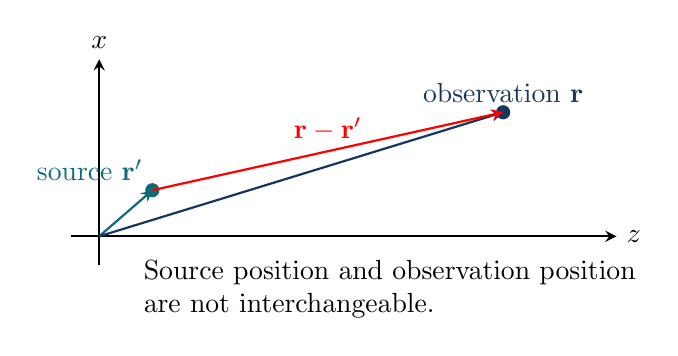
\begin{tikzpicture}[>=stealth,scale=.9]
\draw[->,thick] (-.4,0)--(7.3,0) node[right] {$z$};
\draw[->,thick] (0,-.4)--(0,2.5) node[above] {$x$};
\fill[teal] (.75,.65) circle (.10) node[above left] {source $\mathbf r'$};
\fill[navy] (5.7,1.75) circle (.10) node[above] {observation $\mathbf r$};
\draw[->,thick,teal] (0,0)--(.75,.65);
\draw[->,thick,navy] (0,0)--(5.7,1.75);
\draw[->,thick,red] (.75,.65)--(5.7,1.75) node[midway,above] {$\mathbf r-\mathbf r'$};
\node[align=left] at (4.1,-.75) {Source position and observation position\\are not interchangeable.};
\end{tikzpicture}
\end{center}
\section*{1. The six-step procedure from the lecture}
For an azimuthally symmetric distribution (independent of $\phi'$), the source moments and exterior potential are
\begin{result}{Core formulas: $r>R_{\max}$}
\[\boxed{Q_n=\int r'^nP_n(\cos\theta')\,\dd Q},\qquad\boxed{V(r,\theta)=\frac{1}{4\pi\eps}\sum_{n=0}^\infty\frac{Q_n}{r^{n+1}}P_n(\cos\theta)}.\]
\end{result}
Here $(r',\theta',\phi')$ locates a \emph{source charge}; $(r,\theta,\phi)$ locates the \emph{observation point}; $P_n$ is the Legendre polynomial; and $R_{\max}$ is the greatest source distance from the origin. The expansion is valid outside a sphere containing the entire source, not automatically everywhere outside the physical material.
\begin{enumerate}[label=\textbf{Step \arabic*.},itemsep=3pt]
\item Describe the charge distribution: volume density $\rho(\mathbf r')$, line density $\lambda$, or discrete point charges.
\item Find $R_{\max}$.
\item Choose the appropriate charge element: $\dd Q=\rho\,\dd\tau'$, $\dd Q=\lambda\,\dd\ell'$, or a finite sum of point charges.
\item Evaluate $Q_n=\int r'^nP_n(\cos\theta')\dd Q$ over \emph{all} charge.
\item Substitute the moments into the exterior potential series.
\item Expand the first few \emph{nonzero} terms; use symmetry to eliminate zero terms before calculating.
\end{enumerate}
\begin{insight}{Before using the compact summation}
The series is just an ordered list of contributions:
\[V(r,\theta)=\frac{1}{4\pi\eps}\left[\underbrace{\frac{Q_0}{r}}_{\text{monopole}}+\underbrace{\frac{Q_1}{r^2}\cos\theta}_{\text{dipole}}+\underbrace{\frac{Q_2}{r^3}P_2(\cos\theta)}_{\text{quadrupole}}+\cdots\right].\]
The symbol $n$ labels which angular pattern we are calculating. We compute one $Q_n$ at a time; no index manipulation is required to solve these examples. The charge element $\dd Q$ describes the actual physical source (point, line, ring, or volume), whereas $Q_n$ describes a \emph{moment} of that source. They are not the same quantity.
\end{insight}
Useful identities:
\[P_0(x)=1,\quad P_1(x)=x,\quad P_2(x)=\tfrac12(3x^2-1),\quad P_3(x)=\tfrac12(5x^3-3x),\quad P_4(x)=\tfrac18(35x^4-30x^2+3).\]
\[P_n(1)=1,\qquad P_n(-1)=(-1)^n,\qquad P_{2k+1}(0)=0,\qquad P_2(0)=-\tfrac12,\quad P_4(0)=\tfrac38.\]
\begin{insight}{Why these formulas work}
The Coulomb kernel expands as $|\mathbf r-\mathbf r'|^{-1}=\sum_{n\ge0}(r'^n/r^{n+1})P_n(\cos\gamma)$ for $r>r'$, where $\gamma$ is the angle between source and observation directions. Integration over source azimuth for an axisymmetric distribution leaves $P_n(\cos\theta)P_n(\cos\theta')$. The formula above already incorporates that angular reduction.
\end{insight}
\begin{insight}{Choosing the source element without guessing}
A point charge is handled by a finite sum. A wire uses $\dd Q=\lambda\,\dd\ell'$. A ring uses $\dd\ell'=a\,\dd\phi'$. A three-dimensional cloud uses $\dd Q=\rho\,\dd\tau'$ with $\dd\tau'=r'^2\sin\theta'\,\dd r'\,\dd\theta'\,\dd\phi'$. Before finding any multipole moment, integrate $\dd Q$ alone: the result must be the stated net charge.
\end{insight}
\section*{2. Example 1 --- point charge at the origin}
\textbf{Original problem statement.} ``A charge distribution consists of a point charge $+q$ located at the origin. Find the multipole expansion of the potential, and provide the first few non-zero terms.''

\textbf{Step 1:} The charge density is $\rho(\mathbf r')=q\delta^{(3)}(\mathbf r')$. The three-dimensional delta function picks out the origin; it is not an ordinary function of $r'$ alone.

\textbf{Step 2:} $R_{\max}=0$.

\textbf{Step 3:} $\dd Q=\rho(\mathbf r')\dd\tau'$; in spherical coordinates $\dd\tau'=r'^2\sin\theta'\dd r'\dd\theta'\dd\phi'$.

\textbf{Step 4:} The delta-function sifting property gives
\[Q_n=\int r'^nP_n(\cos\theta')q\delta^{(3)}(\mathbf r')\dd\tau'.\]
For $n=0$, $r'^0P_0=1$, so $Q_0=q$. For every $n\ge1$, the factor $r'^n$ vanishes at the origin, so $Q_n=0$. Although $\theta'$ is undefined precisely at the origin, $r'^nP_n(\cos\theta')$ has the continuous value zero there for $n\ge1$.

\textbf{Steps 5--6:} Only the monopole survives:
\begin{result}{Point charge result}\[\boxed{V(r)=\frac{q}{4\pi\eps r},\qquad r>0.}\]\end{result}
\textbf{Check:} The potential is angle-independent, as spherical symmetry requires.
\begin{insight}{What should we predict for a charge at the origin?}
Every source position has distance $r'=0$ from the chosen origin. The monopole measures net charge, but every higher moment carries at least one power of source distance. Therefore all higher moments vanish. The choice of origin matters: moving the same point charge away from the origin generally produces higher moments about the new origin.
\end{insight}
\section*{3. Example 2 --- two equal and opposite axial charges}
\textbf{Original problem statement.} ``A charge distribution consists of a charge $+q$ at $z=+d/2$ on the $z$-axis and another charge $-q$ located on the $z$-axis at $z=-d/2$. Find the multipole expansion of the potential, and provide the first few non-zero terms.''

\begin{center}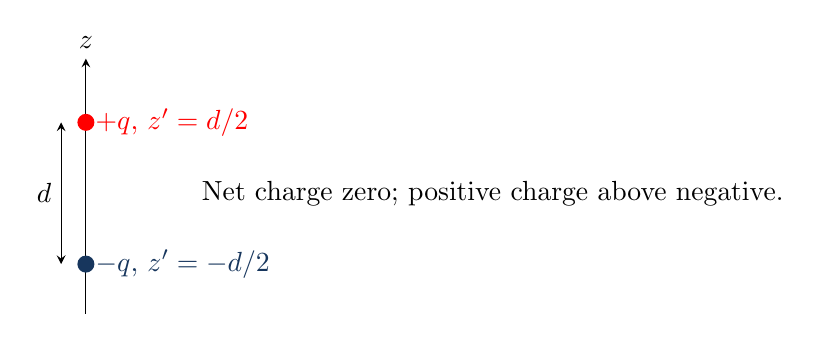
\begin{tikzpicture}[>=stealth,scale=.9]
\draw[->] (0,-1.7)--(0,1.9) node[above] {$z$};
\fill[red] (0,1) circle (.12) node[right] {$+q$, $z'=d/2$};
\fill[navy] (0,-1) circle (.12) node[right] {$-q$, $z'=-d/2$};
\draw[<->] (-.35,-1)--(-.35,1) node[midway,left] {$d$};
\node[right] at (1.5,0) {Net charge zero; positive charge above negative.};
\end{tikzpicture}\end{center}
\textbf{Step 1:} The charges are at $\mathbf r'_+=\tfrac d2\hat{\mathbf z}$ and $\mathbf r'_-=-\tfrac d2\hat{\mathbf z}$:
\[\rho(\mathbf r')=q\delta^{(3)}(\mathbf r'-\mathbf r'_+)-q\delta^{(3)}(\mathbf r'-\mathbf r'_-).\]
\textbf{Step 2:} $R_{\max}=d/2$.

\textbf{Step 3:} Use the discrete charge elements $+q$ and $-q$ (equivalent to integrating the delta functions).

\textbf{Step 4:} Both have $r'=d/2$, but their polar angles are $0$ and $\pi$. Thus
\begin{align*}Q_n&=q(d/2)^nP_n(\cos0)-q(d/2)^nP_n(\cos\pi)\\
&=q(d/2)^n[P_n(1)-P_n(-1)]\\
&=q(d/2)^n[1-(-1)^n].\end{align*}
For even $n$, $(-1)^n=1$ and the moments cancel. For odd $n$, $(-1)^n=-1$ and the moments add:
\[\boxed{Q_n=\begin{cases}0,&n\text{ even},\\\dfrac{qd^n}{2^{n-1}},&n\text{ odd}.\end{cases}}\]
\textbf{Steps 5--6:} $Q_1=qd$, $Q_3=qd^3/4$, $Q_5=qd^5/16$:
\begin{result}{Axial dipole expansion, $r>d/2$}
\[\boxed{V(r,\theta)=\frac{1}{4\pi\eps}\left[\frac{qd\cos\theta}{r^2}+\frac{qd^3}{4r^4}P_3(\cos\theta)+\frac{qd^5}{16r^6}P_5(\cos\theta)+\cdots\right].}\]
\end{result}
The monopole vanishes because the total charge is zero. The leading term is the dipole with $p_z=qd$. Reflection $z\mapsto-z$ reverses the charge distribution, so only odd Legendre modes remain.
\begin{insight}{Why does the dipole term survive?}
The upper charge contributes $+q(d/2)$ to $Q_1$. The lower charge contributes $(-q)(-d/2)=+qd/2$. Their sum is $qd$. Notice that the \emph{charge signs} and \emph{position signs} both matter. For the monopole, $+q-q=0$. For the next even moment, both positions are squared and the charges cancel again.
\end{insight}
\section*{4. Example 3 --- spherically symmetric charged sphere}
\textbf{Original problem statement.} ``A charge $+q$ is distributed as $\rho(r')=f(r')$ in a sphere of radius $a$. The sphere is centered on the origin. Find the multipole expansion of the potential, and provide the first few non-zero terms.''

\textbf{Steps 1--3:} $\rho(r',\theta')=f(r')P_0(\cos\theta')=f(r')$ for $0\le r'\le a$, $R_{\max}=a$, and
\[\dd Q=f(r')r'^2\sin\theta'\dd r'\dd\theta'\dd\phi'.\]
\textbf{Step 4:} Substitute into the moment integral and separate independent integrations:
\begin{align*}
Q_n&=\int_0^a f(r')r'^{n+2}\dd r'\int_0^{2\pi}\dd\phi'\int_0^\pi P_n(\cos\theta')\sin\theta'\dd\theta'\\
&=2\pi\left[\int_0^a f(r')r'^{n+2}\dd r'\right]\left[\int_{-1}^{1}P_n(u)\dd u\right].
\end{align*}
The substitution $u=\cos\theta'$ yields $\dd u=-\sin\theta'\dd\theta'$ and reverses the integration limits. Orthogonality with $P_0(u)=1$ gives
\[\int_{-1}^1P_n(u)P_0(u)\dd u=\frac{2}{2n+1}\delta_{n0}.\]
Therefore $Q_n=0$ for $n\ge1$, while
\[Q_0=4\pi\int_0^a f(r')r'^2\dd r'=q.\]
\textbf{Steps 5--6:} The entire exterior series collapses to one term:
\begin{result}{Exterior potential of any spherical charge cloud}
\[\boxed{V(r)=\frac{q}{4\pi\eps r},\qquad r>a.}\]
\end{result}
\textbf{Important distinction:} This result describes the \emph{exterior} potential. The interior potential depends on the radial density $f(r')$; it is not generally $q/(4\pi\eps r)$ for $r<a$.
\begin{insight}{Why the angular integral disappears}
The density $f(r')$ has no angular preference. For the monopole, $P_0=1$, so integrating over all directions gives $4\pi$. For every higher Legendre pattern, positive and negative angular lobes cancel when averaged over a full sphere. This is the mathematical version of the physical fact that a spherical charge cloud looks like a point charge from outside.
\end{insight}
\section*{5. Example 4 --- uniformly charged circular ring}
\textbf{Original problem statement.} ``A charge $+q$ is uniformly distributed on an infinitesimally thin ring of radius $a$. The ring lies in the $xy$-plane centered on the origin. Find the multipole expansion of the potential, and provide the first few non-zero terms.''

\begin{center}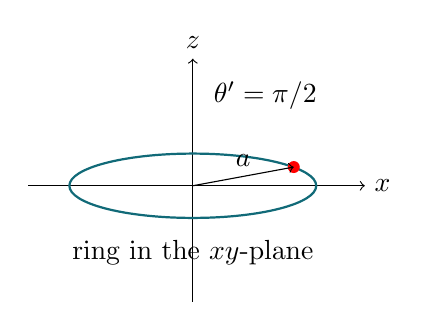
\begin{tikzpicture}[scale=.95]
\draw[->] (-2.2,0)--(2.3,0) node[right] {$x$};
\draw[->] (0,-1.55)--(0,1.7) node[above] {$z$};
\draw[thick,teal] (0,0) ellipse (1.65 and .43);
\fill[red] (1.35,.25) circle (.08);
\draw[->] (0,0)--(1.35,.25) node[midway,above] {$a$};
\node[below] at (0,-.6) {ring in the $xy$-plane};
\node[right] at (.15,1.2) {$\theta'=\pi/2$};
\end{tikzpicture}\end{center}
\textbf{Steps 1--3:} All source points satisfy $r'=a$, $\theta'=\pi/2$, and $0\le\phi'<2\pi$. The linear density is
\[\lambda=\frac{q}{2\pi a},\qquad R_{\max}=a,\qquad\dd Q=\lambda a\dd\phi'=\frac{q}{2\pi}\dd\phi'.\]
\textbf{Step 4:} Substitute the constant radius and polar angle:
\begin{align*}Q_n&=\int_0^{2\pi}a^nP_n(\cos(\pi/2))\frac{q}{2\pi}\dd\phi'\\
&=\frac{qa^nP_n(0)}{2\pi}(2\pi)=qa^nP_n(0).
\end{align*}
Because $P_n(0)=0$ for odd $n$, all odd moments vanish. For the first even moments,
\[Q_0=q,\qquad Q_2=-\frac{qa^2}{2},\qquad Q_4=\frac{3qa^4}{8}.\]
\textbf{Steps 5--6:} Substitute each moment into the potential series:
\begin{result}{Ring expansion, $r>a$}
\[\boxed{V(r,\theta)=\frac{q}{4\pi\eps r}\left[1-\frac12\left(\frac ar\right)^2P_2(\cos\theta)+\frac38\left(\frac ar\right)^4P_4(\cos\theta)+\cdots\right].}\]
\end{result}
\textbf{Check on the axis:} At $\theta=0$, $P_n(1)=1$, so
\[V(r,0)=\frac{q}{4\pi\eps r}\left[1-\frac{a^2}{2r^2}+\frac{3a^4}{8r^4}+\cdots\right].\]
This agrees with the large-$r$ binomial expansion of the exact axial ring potential $q/[4\pi\eps\sqrt{r^2+a^2}]$. Reflection symmetry about the $xy$-plane forbids odd moments.
\begin{insight}{Why the ring quadrupole is negative}
For every charge element, the source polar angle is $90^\circ$, so $\cos\theta'=0$. Evaluate the second Legendre polynomial directly:
\[P_2(0)=\frac12\big(3(0)^2-1\big)=-\frac12.\]
Multiplying by the positive total charge and $a^2$ gives $Q_2=-qa^2/2$. The negative sign is a geometric signature of charge concentrated around the equatorial plane, not a negative physical charge.
\end{insight}
\section*{6. Example 5 --- uniformly charged finite line on the $z$-axis}
\textbf{Original problem statement.} ``A finite thin line of length $2a$ and charge $+q$ lies on the $z$-axis from $z=-a$ to $z=+a$. Find the multipole expansion of the potential, and provide the first few non-zero terms.''

\textbf{Note on the slides:} The problem is labeled ``Example 5'' on slide 19 but ``Example 4'' in the header of slide 20. It is the fifth distinct example in this lecture.

\begin{center}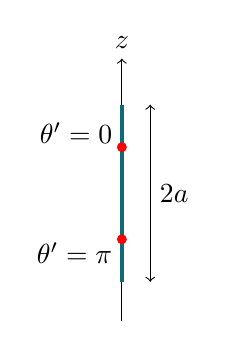
\begin{tikzpicture}[scale=.9]
\draw[->] (0,-1.8)--(0,1.9) node[above] {$z$};
\draw[very thick,teal] (0,-1.25)--(0,1.25);
\draw[<->] (.4,-1.25)--(.4,1.25) node[midway,right] {$2a$};
\fill[red] (0,.65) circle (.07);
\fill[red] (0,-.65) circle (.07);
\node[left] at (0,.85) {$\theta'=0$};
\node[left] at (0,-.85) {$\theta'=\pi$};
\end{tikzpicture}\end{center}
\textbf{Steps 1--3:} The constant line density and maximum source radius are
\[\lambda=\frac{q}{2a},\qquad R_{\max}=a,\qquad\dd Q=\lambda\dd z'.\]
To follow the lecture's two-piece treatment, let $r'=|z'|$. On the upper half $\theta'=0$, so $P_n(\cos\theta')=P_n(1)$. On the lower half $\theta'=\pi$, so $P_n(\cos\theta')=P_n(-1)$. Each half uses $0\le r'\le a$.

\textbf{Step 4:} Add the two contributions:
\begin{align*}
Q_n&=\lambda\int_0^a r'^nP_n(1)\dd r'+\lambda\int_0^a r'^nP_n(-1)\dd r'\\
&=\lambda[1+(-1)^n]\int_0^a r'^n\dd r'\\
&=\lambda[1+(-1)^n]\left[\frac{r'^{n+1}}{n+1}\right]_{0}^{a}\\
&=\frac{\lambda a^{n+1}}{n+1}[1+(-1)^n].
\end{align*}
For odd $n$ the bracket is zero; for even $n$ it equals $2$. Substitute $\lambda=q/(2a)$:
\[\boxed{Q_n=\begin{cases}\dfrac{qa^n}{n+1},&n\text{ even},\\0,&n\text{ odd}.\end{cases}}\]
In particular, $Q_0=q$, $Q_2=qa^2/3$, and $Q_4=qa^4/5$.

\textbf{Steps 5--6:} Only even powers appear:
\begin{result}{Finite-line expansion, $r>a$}
\[\boxed{V(r,\theta)=\frac{q}{4\pi\eps r}\left[1+\frac13\left(\frac ar\right)^2P_2(\cos\theta)+\frac15\left(\frac ar\right)^4P_4(\cos\theta)+\cdots\right].}\]
\end{result}
\textbf{Check:} $Q_0=q$, and the $n=2$ coefficient is positive because charge lies along the polar axis, in contrast with the ring in the equatorial plane.
\begin{insight}{Why the line quadrupole is positive}
Both halves of the wire lie on the polar axis, where $P_2(1)=P_2(-1)=1$. Unlike the ring, every element contributes positively to $Q_2$. The two halves also show why odd moments cancel: the upper and lower elements have equal charge and equal distance, but opposite odd Legendre factors.
\end{insight}
\section*{7. Compare the five examples}
\begin{center}\small\begin{tabular}{p{.27\linewidth}p{.14\linewidth}p{.19\linewidth}p{.28\linewidth}}\toprule
Distribution & $R_{\max}$ & Nonzero $n$ & Leading exterior potential\\\midrule
Point $+q$ at origin & $0$ & $0$ only & $q/(4\pi\eps r)$\\
Opposite charges $\pm q$ & $d/2$ & odd & $qd\cos\theta/(4\pi\eps r^2)$\\
Spherical $f(r')$ & $a$ & $0$ only & $q/(4\pi\eps r)$\\
Circular ring & $a$ & even & $q/(4\pi\eps r)$\\
Centered axial line & $a$ & even & $q/(4\pi\eps r)$\\\bottomrule
\end{tabular}\end{center}
\begin{insight}{Symmetry test before integration}
A charge distribution invariant under $z\mapsto-z$ has no odd axial multipole moments. A distribution that reverses sign under that reflection has no even moments. Full spherical symmetry eliminates \emph{all} moments beyond the monopole. For a nonzero total charge, the monopole dominates far away even if higher moments are present.
\end{insight}
\begin{insight}{Sanity checks you can perform without integrating}
\textbf{Net charge:} $Q_0$ must equal the total source charge. \textbf{Units:} $Q_n$ has charge times length to the $n$th power, so $Q_n/r^{n+1}$ has units of charge per length. \textbf{Symmetry:} reflection about the equatorial plane removes odd moments when charge is unchanged. \textbf{Far field:} each successive nonzero multipole falls off with one additional power of $1/r$ per step in $n$. \textbf{Domain:} the exterior series is guaranteed only when the observation radius exceeds the largest source radius.
\end{insight}
\section*{8. Superposition and the lecture's final summary}
For a composite system built from multiple axially symmetric parts, charge density adds: $\rho=\rho_1+\rho_2+\cdots$. Because integration is linear,
\[\boxed{Q_n^{\mathrm{total}}=\sum_jQ_n^{(j)}},\qquad\boxed{V_{\mathrm{total}}=\sum_jV_j}.\]
Choose a \emph{common origin and axis} when adding moments. For example, a concentric spherical cloud and ring contribute $Q_0=q_{\rm sphere}+q_{\rm ring}$, while $Q_2$ comes only from the ring; axial point charges can contribute additional odd moments. Each exterior expansion requires $r$ greater than the largest source radius in the \emph{combined} configuration.

\textbf{Far-field hierarchy:}
\[V(r,\theta)=\frac{1}{4\pi\eps}\left[\frac{Q_0}{r}+\frac{Q_1\cos\theta}{r^2}+\frac{Q_2P_2(\cos\theta)}{r^3}+\cdots\right].\]
If $Q_0\ne0$, the leading term is the monopole $Q_0/(4\pi\eps r)$. If $Q_0=0$ and $Q_1\ne0$, the leading term is the dipole $Q_1\cos\theta/(4\pi\eps r^2)$. If both vanish, inspect the quadrupole and higher moments. \emph{A neutral distribution need not have a nonzero dipole}; its first surviving term may occur at $n=2$ or higher.
\begin{result}{Exam checklist}
\begin{enumerate}[leftmargin=*,itemsep=2pt]
\item Write the source geometry and its $\dd Q$ correctly; normalize it to the given total charge.
\item Determine $R_{\max}$ and state the valid exterior region.
\item Use $P_n(1)$, $P_n(-1)$, $P_n(0)$ and reflection symmetry to identify vanishing terms.
\item Integrate to find $Q_n$; check $Q_0$ equals the net charge and $[Q_n]=\mathrm{C\,m^n}$.
\item Substitute into $V$ and display the first three surviving terms (or explain why only one exists).
\end{enumerate}
\end{result}
\end{document}
